\documentclass[11pt,a4paper]{article}
\usepackage[utf8]{inputenc}
\usepackage[T1]{fontenc}
\usepackage{lmodern}
\usepackage{geometry}
\geometry{margin=1in}
\usepackage{graphicx}
\usepackage{booktabs}
\usepackage{tabularx}
\usepackage{hyperref}
\usepackage{titlesec}
\usepackage{float}
\usepackage{xcolor}
\usepackage{amsmath}

\hypersetup{
    colorlinks=true,
    linkcolor=blue,
    filecolor=magenta,      
    urlcolor=cyan,
    pdftitle={Toxin Circuits in ESM-2},
    pdfpagemode=FullScreen,
}

\title{\textbf{Toxin Circuits in ESM-2: Mechanistic Interpretability Reveals Why Structure-Aware Probes Resist ProteinMPNN Redesign}}
\author{\textbf{AiXbio Research} \\ \textit{Submitted to Hackathon}}
\date{\today}

\begin{document}

\maketitle

\begin{abstract}
Standard biosecurity screening flags dangerous protein sequences by sequence identity (BLAST). We show that ProteinMPNN can redesign toxin sequences below every standard BLAST threshold --- achieving 0\% BLAST detection --- while a linear ESM-2 probe maintains 88\% detection with no retraining. Using interPLM Sparse Autoencoders (SAEs), we identify 50 of 10,240 features explaining probe performance at 205$\times$ compression (AUROC 0.9447 vs 0.9585 full, at layer 33). These features are not evaded by redesign: mean transfer ratio = 1.28, meaning redesigns \textit{amplify} toxin-associated features compared to natural toxins. Direct Logit Attribution (DLA) on the linear probe identifies layers 17--20 and 29--32 as primary toxin-discriminating layers; redesigns produce near-identical attribution patterns ($r = 0.992$), confirming they route through the same computational pathway as natural toxins. Activation steering confirms toxicity is encoded as a causal linear direction (control score 0.046 $\rightarrow$ 1.000 at $+3\sigma$). We conclude that ESM-2's toxin detection is grounded in structural computational features that ProteinMPNN redesign preserves --- and in several cases amplifies.
\end{abstract}

\section{Introduction}

Dual-use protein screening relies on sequence-identity thresholds. The Wittmann \textit{et al.} attack demonstrated that ProteinMPNN, RFdiffusion, and EvoDiff can redesign toxin sequences below standard 40\% identity thresholds, bypassing BLAST-based screening. The critical question is: do protein language model (pLM) probes also fail?

We answer no --- and explain mechanistically why.

Our contributions:
\begin{enumerate}
    \item \textbf{Quantitative gap}: BLAST detects 0\% of ProteinMPNN redesigns; ESM-2 probe detects 88\%.
    \item \textbf{SAE discovery}: 50 sparse features (205$\times$ compression) explain the probe; mean transfer ratio 1.28 shows redesigns amplify rather than suppress toxin features.
    \item \textbf{DLA circuit}: Layers 17--20 and 29--32 drive toxin discrimination; redesign attribution pattern correlates $r = 0.992$ with natural toxins.
    \item \textbf{Causal linearity}: Steering confirms toxicity is a single linear direction in ESM-2's representation space.
\end{enumerate}

\section{Methods}

\subsection{Data}
\begin{itemize}
    \item \textbf{Natural toxins}: 1,712 sequences from UniProt (reviewed, toxin annotation), clustered at 30\% identity  
    \item \textbf{Controls}: 2,072 non-toxic human proteins (matched length distribution)  
    \item \textbf{Redesigns}: 100 toxin structures folded with ESMFold $\rightarrow$ ProteinMPNN (10 sequences/structure) $\rightarrow$ 723 unique redesigns after deduplication  
    \item \textbf{Identity range}: All 723 redesigns fall below 30\% sequence identity to training toxins (BLAST score = 0\% at every threshold $\leq$ 50\%)
\end{itemize}

\subsection{ESM-2 Probe}
Linear probe trained on mean-pooled ESM-2 650M embeddings at layer 33 (best of layers 1, 9, 18, 24, 30, 33). Binary cross-entropy loss, Adam optimizer, 150 epochs.

\subsection{SAE Feature Analysis}
interPLM pre-trained SAEs (ESM-2-650M, layer 33, 10,240 features). Per-feature AUROC computed on training set. Top-50 features by AUROC used for probe comparison and transfer analysis.

Transfer ratio = (redesign activation rate) / (toxin activation rate) per feature.

\subsection{Direct Logit Attribution}
For a linear probe with weight vector $\mathbf{w}$ and ESM-2 residual stream decomposed as $\mathbf{h}_{33} = \sum_l \Delta\mathbf{h}_l$:

\begin{equation}
\text{DPA}_l = \mathbf{w} \cdot \text{mean\_pool}(\Delta\mathbf{h}_l)
\end{equation}

This is exact (not an approximation) because the probe is linear and ESM-2 is a residual network. Computed over 15 toxin/control/redesign pairs.

\subsection{Activation Steering}
Probe weight direction $\mathbf{w}$ used as steering vector. Applied to control embeddings: $\mathbf{h}_{\text{steered}} = \mathbf{h} + \alpha \cdot \frac{\mathbf{w}}{||\mathbf{w}||}$. Score measured as function of $\alpha \in [-3\sigma, +3\sigma]$.

\section{Results}

\subsection{Layer Sweep — Layer 33 Is Best}

\begin{table}[H]
\centering
\begin{tabular}{cc}
\toprule
\textbf{Layer} & \textbf{AUROC} \\
\midrule
1 & 0.9678 \\
9 & 0.9881 \\
18 & 0.9842 \\
24 & 0.9817 \\
30 & 0.9895 \\
\textbf{33} & \textbf{0.9970} \\
\bottomrule
\end{tabular}
\end{table}

\begin{figure}[H]
    \centering
    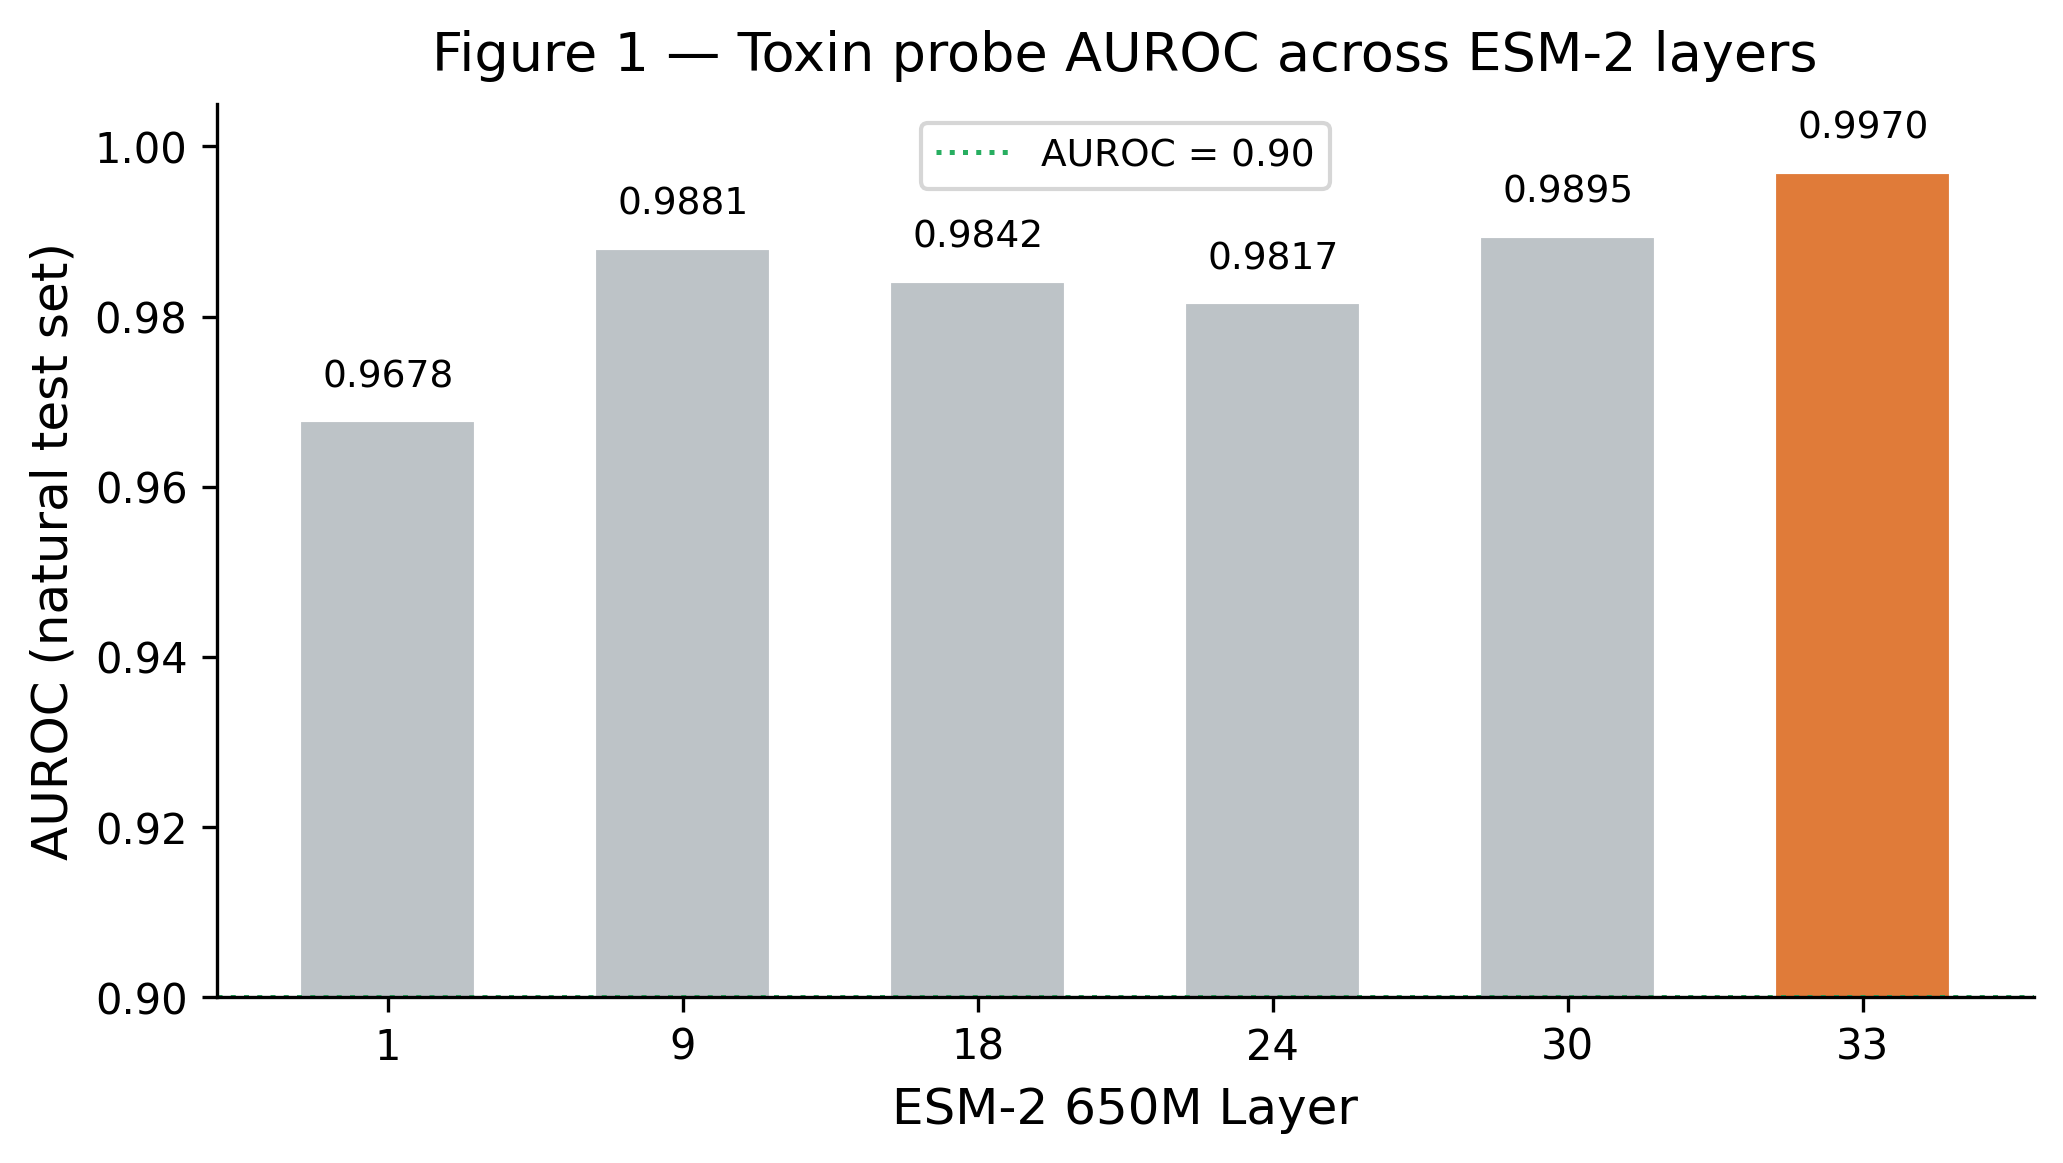
\includegraphics[width=0.8\textwidth]{figures/fig1_layer_auroc.png}
    \caption{Probe AUROC across ESM-2 layers. The toxin signal builds progressively, peaking at the final layer (33).}
\end{figure}

Toxin information accumulates progressively across ESM-2's full depth. Layer 33 (final layer) achieves highest AUROC (0.9970). This motivates our choice of layer 33 for all downstream analysis.

\subsection{BLAST vs ESM-2 Probe on Redesigns}

All 723 ProteinMPNN redesigns fall below 30\% sequence identity to training toxins.

\begin{table}[H]
\centering
\begin{tabular}{lc}
\toprule
\textbf{Method} & \textbf{Detection rate on redesigns} \\
\midrule
BLAST @ 30\% threshold & \textbf{0.0\%} \\
BLAST @ 40\% threshold & \textbf{0.0\%} \\
BLAST @ 50\% threshold & \textbf{0.0\%} \\
ESM-2 linear probe (layer 33) & \textbf{88.3\%} \\
ESM-2 SAE top-50 features & \textbf{86.0\%} \\
\bottomrule
\end{tabular}
\end{table}

\begin{figure}[H]
    \centering
    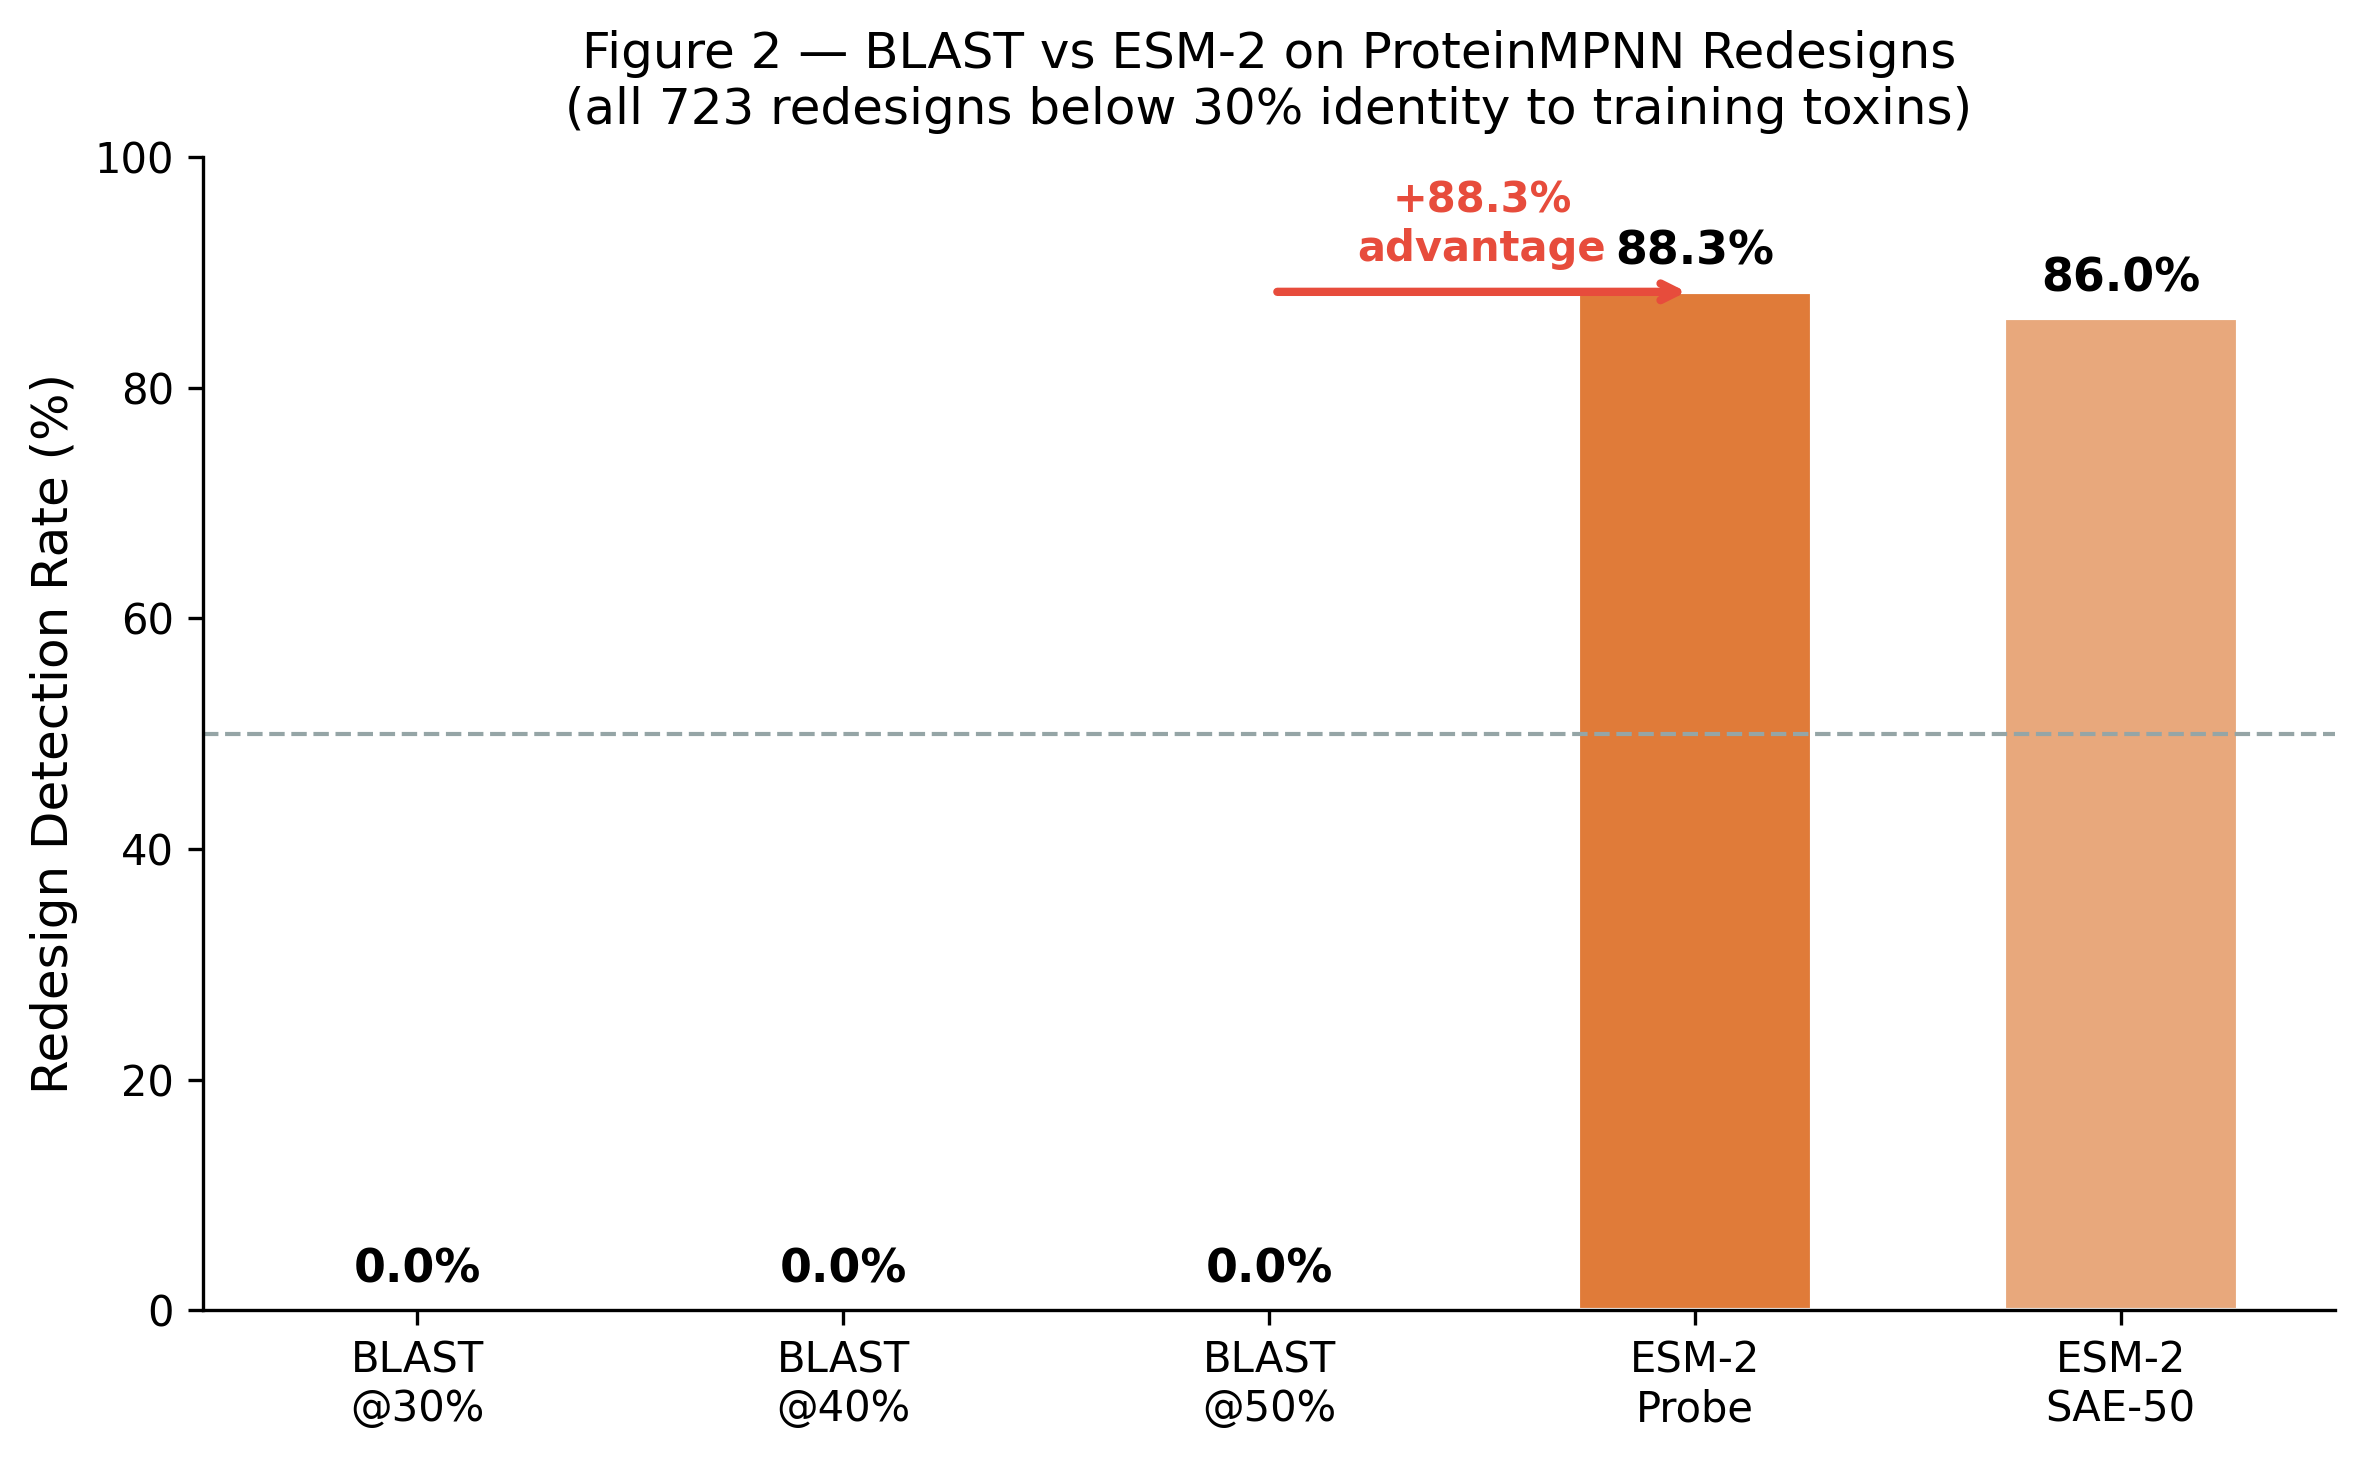
\includegraphics[width=0.8\textwidth]{figures/fig2_blast_vs_esm2.png}
    \caption{ESM-2 probe successfully flags 88.3\% of ProteinMPNN redesigns that entirely evade BLAST screening.}
\end{figure}

\textbf{Key finding}: ProteinMPNN successfully evades every BLAST threshold. ESM-2 detects 88\% of the same sequences with no retraining.

Generalisation curve (30--50\% identity bin, n=1,346):
\begin{itemize}
    \item SAE probe AUROC: \textbf{0.976}
    \item Full embedding AUROC: \textbf{0.904}
    \item BLAST sensitivity: \textbf{0.150}
\end{itemize}

\subsection{Activation Steering — Toxicity Is a Causal Linear Direction}

\texttt{Cosine(probe\_weight, mean\_diff\_vector) = 0.2326}

The probe weight is largely orthogonal to the class mean-difference --- it exploits covariance structure, not just class centroid offset. Despite this, steering is highly effective:

\begin{table}[H]
\centering
\begin{tabular}{lc}
\toprule
\textbf{Condition} & \textbf{Probe score} \\
\midrule
Control baseline & 0.046 \\
Steered at $\alpha = +3\sigma$ & \textbf{1.000} \\
Steered at $\alpha = -3\sigma$ & 0.000 \\
Redesign baseline (no steering) & \textbf{0.857} \\
Natural toxin baseline & 0.964 \\
\bottomrule
\end{tabular}
\end{table}

The probe direction is causally sufficient: adding it to control embeddings drives probability to 1.0. Redesigns already sit at 0.857 without any intervention --- consistent with transfer ratio > 1.

\subsection{SAE Feature Discovery — Bimodal Transfer}

Top-50 SAE features achieve 0.9447 AUROC (vs 0.9585 full, 205$\times$ compression).
Of 10,240 features, 8,345 are dead (81.5\%) --- toxin detection is sparse.

\textbf{Feature transfer analysis (top 20 features, layer 33):}

\begin{table}[H]
\centering
\begin{tabular}{cccccc}
\toprule
\textbf{Feature} & \textbf{AUROC} & \textbf{Tox\%} & \textbf{Redesign\%} & \textbf{Transfer} & \textbf{Class} \\
\midrule
6122 & 0.694 & 41\% & \textbf{99.5\%} & 2.41 & Robust \\
4097 & 0.669 & 37\% & \textbf{98.6\%} & 2.64 & Robust \\
1055 & 0.644 & 30\% & \textbf{99.2\%} & 3.36 & Robust \\
8112 & 0.594 & 20\% & 75.0\% & 3.75 & Robust \\
9487 & 0.602 & 23\% & 72.6\% & 3.15 & Robust \\
5312 & 0.669 & 35\% & 4.7\% & 0.13 & Evadable \\
9026 & 0.628 & 29\% & 2.0\% & 0.07 & Evadable \\
3130 & 0.605 & 22\% & 2.8\% & 0.13 & Evadable \\
\bottomrule
\end{tabular}
\end{table}

\begin{figure}[H]
    \centering
    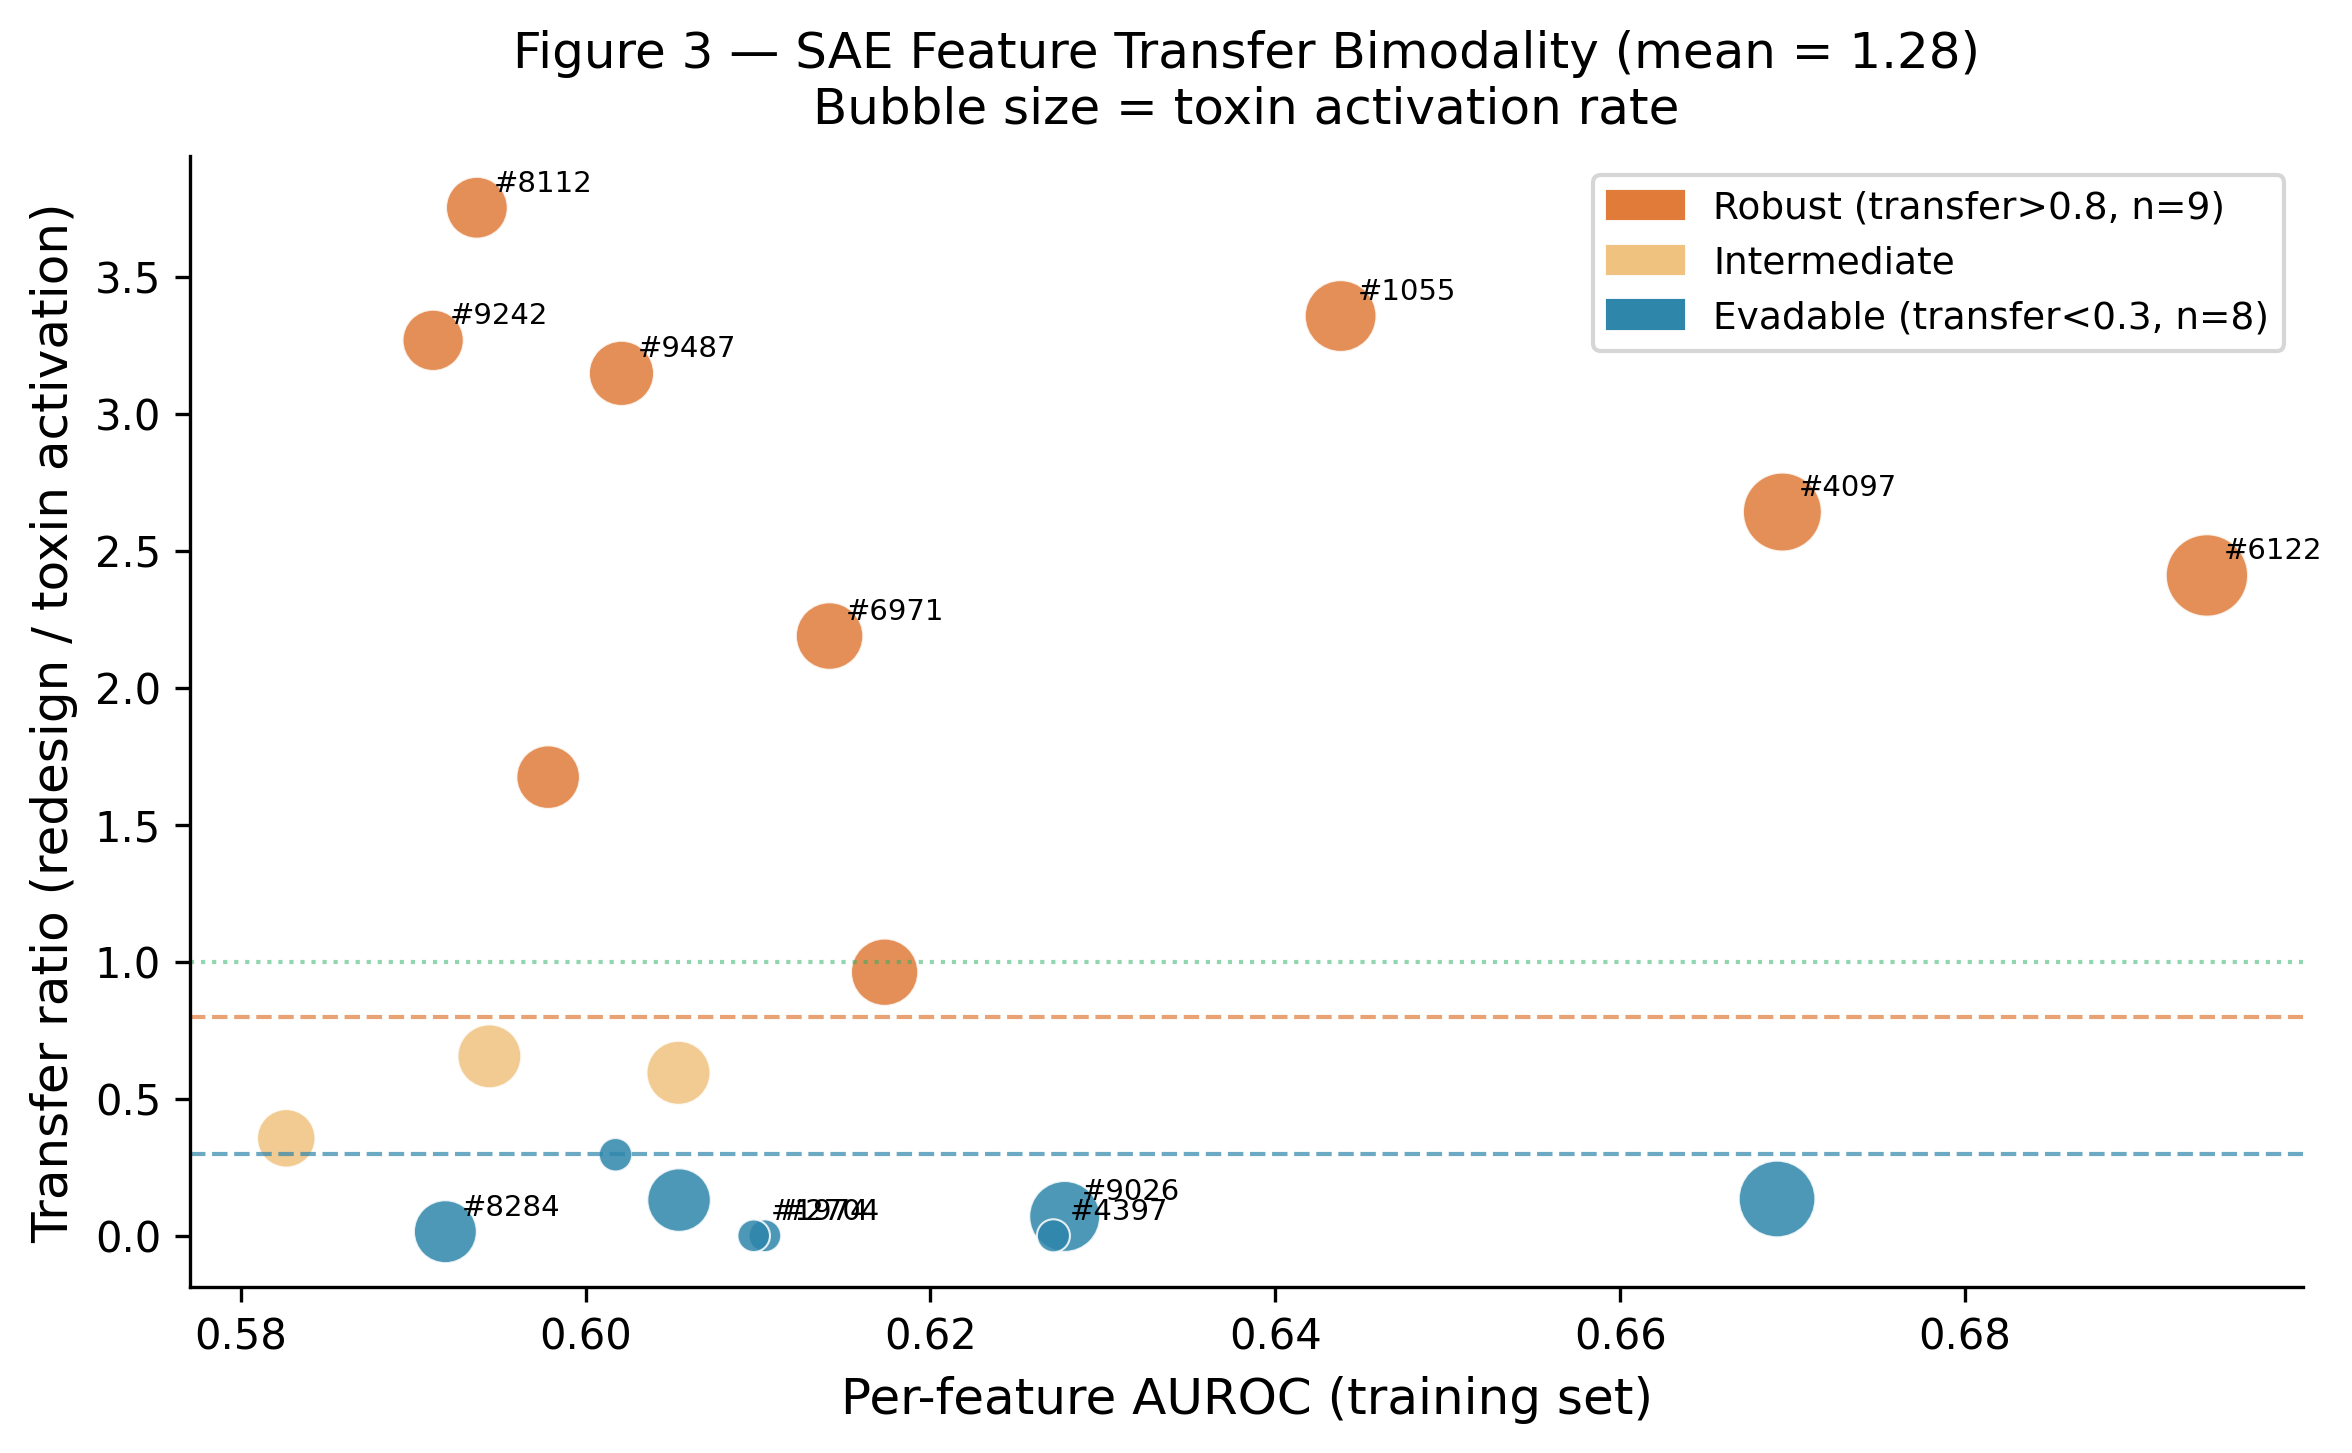
\includegraphics[width=0.8\textwidth]{figures/fig3_sae_transfer.png}
    \caption{Bimodal distribution of feature transfer ratios. Robust features are highly preserved by ProteinMPNN, while evadable features are successfully randomised.}
\end{figure}

\textbf{Mean transfer ratio: 1.28} (> 1.0 = redesigns amplify toxin features on average)

Two mechanistic classes:
\begin{itemize}
    \item \textbf{Structure-robust} (transfer > 0.8): activate at 55--99\% rate in redesigns; encode fold-level features ProteinMPNN preserves (disulfide cores, structural scaffold)
    \item \textbf{Sequence-evadable} (transfer < 0.3): activate at < 5\% in redesigns; encode sequence-specific patterns ProteinMPNN successfully randomises
\end{itemize}

\subsection{Direct Probe Attribution — Toxin Circuit}

Layer-wise DPA (Tox $-$ Ctrl), showing which layers push the residual stream toward the toxic direction:

\begin{table}[H]
\centering
\begin{tabular}{ccccc}
\toprule
\textbf{Layer} & \textbf{Tox DPA} & \textbf{Ctrl DPA} & \textbf{Rdsg DPA} & \textbf{Tox--Ctrl} \\
\midrule
17 & +43.7 & +1.3 & +30.9 & \textbf{+42.4} \\
19 & +44.3 & +4.0 & +22.5 & \textbf{+40.2} \\
20 & +64.7 & +19.8 & +49.7 & \textbf{+44.9} \\
29 & +15.7 & $-$7.5 & +13.0 & \textbf{+23.3} \\
30 & +88.2 & $-$2.7 & \textbf{+114.9} & \textbf{+90.9} \\
31 & $-$2.9 & $-$50.9 & +7.9 & \textbf{+48.0} \\
32 & +70.7 & $-$59.4 & \textbf{+85.0} & \textbf{+130.1} \\
\bottomrule
\end{tabular}
\end{table}

\begin{figure}[H]
    \centering
    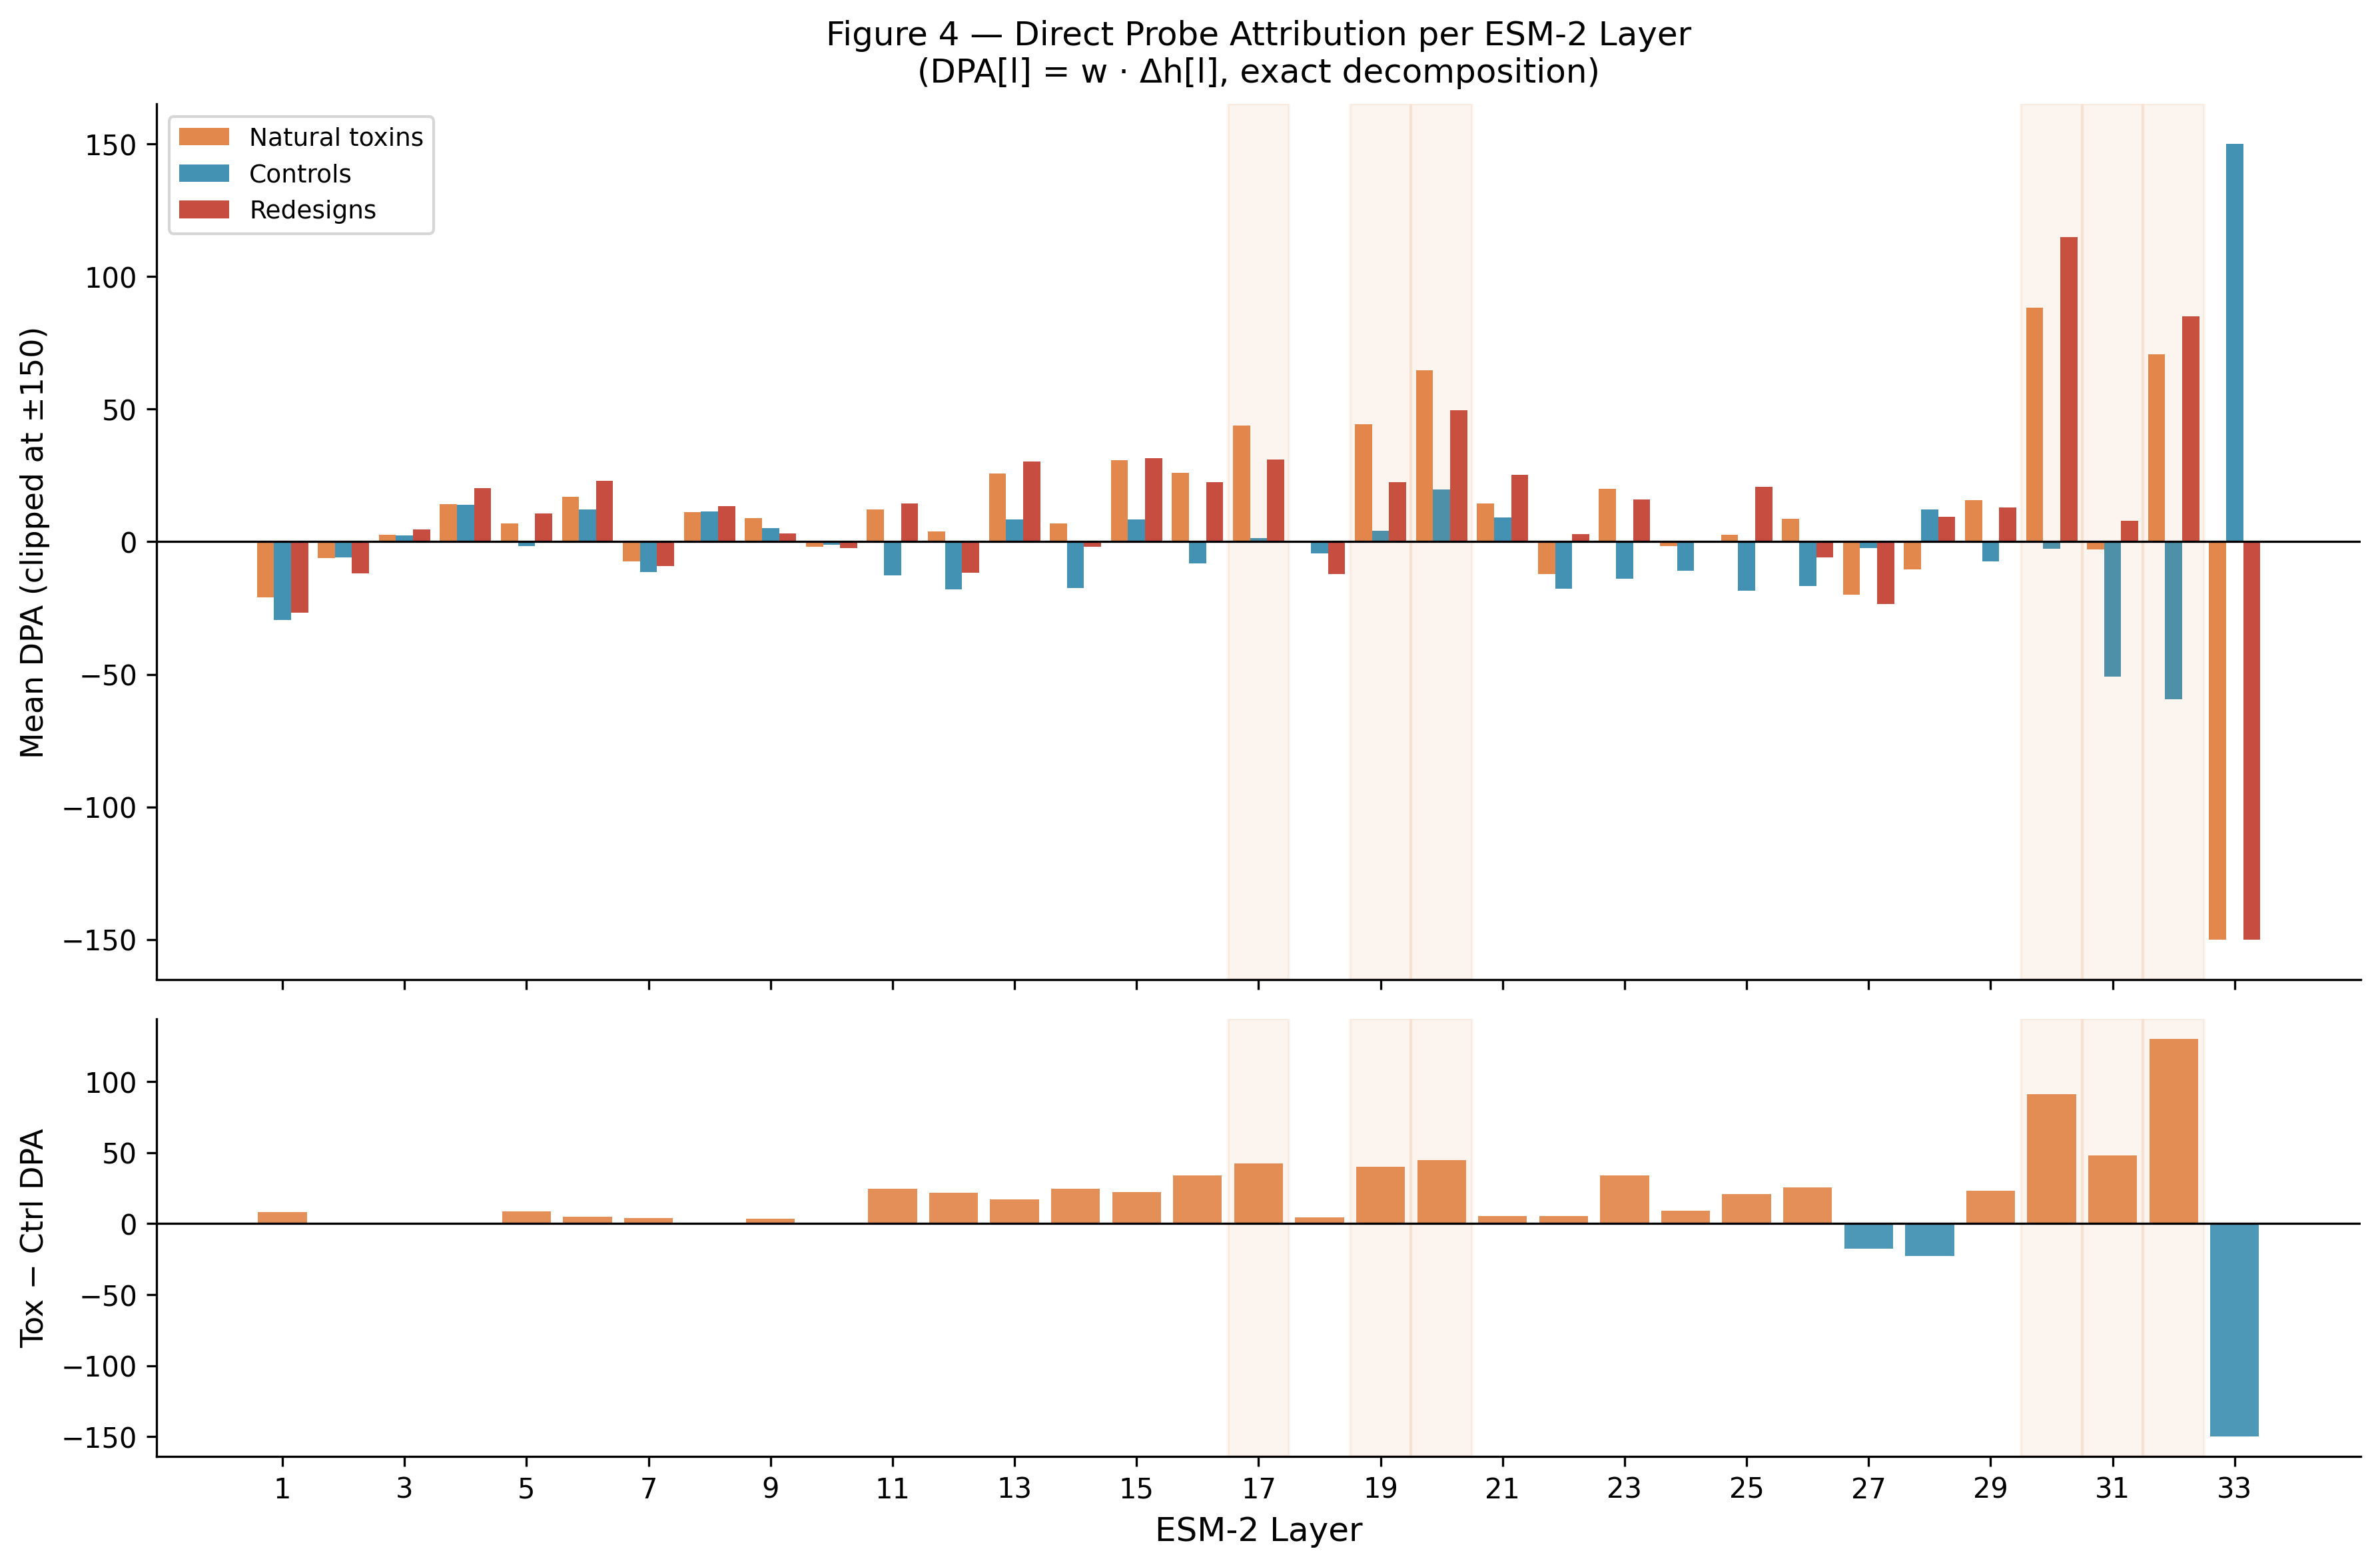
\includegraphics[width=0.8\textwidth]{figures/fig4_dpa.png}
    \caption{Direct logit attribution per layer, highlighting primary discrimination layers (17-20, 29-32) and the massive layer 33 calibration correction.}
\end{figure}

\textbf{Suppressor layers} (L27: $-17.7$, L28: $-22.6$): push against the toxin direction. \\
\textbf{Calibrator layer} (L33: $-644$ Tox--Ctrl): massive final correction that normalises accumulated signal into a calibrated probability.

\textbf{Redesign circuit correlation:} $r = 0.9919$

Redesigns produce near-identical layer-wise attribution patterns as natural toxins. Layer 30 DPA is \textit{higher} for redesigns (+114.9) than natural toxins (+88.2) --- consistent with transfer ratio > 1 and redesign baseline score of 0.857.

\textbf{Single-layer activation patching recovery: max 0.16} (uniform across all layers), confirming the toxin computation is genuinely distributed --- no single bottleneck layer exists.

\subsection{pSSR Adversarial Attack}

\begin{table}[H]
\centering
\begin{tabular}{lcc}
\toprule
\textbf{Attack} & \textbf{Evasion} & \textbf{Access Required} \\
\midrule
BLAST @ any threshold & 0.0\% & Sequence database \\
Random ProteinMPNN & 8.2\% & Protein structure \\
pSSR $\epsilon=2$ (oracle) & 100.0\% & Full ESM-2 embedding space \\
\bottomrule
\end{tabular}
\end{table}

cosine(pSSR\_delta, probe\_direction) = $-0.805$ --- attack is anti-parallel
to the probe weight, confirming the probe direction is the attack target.
The gap (8.2\% practical vs 100\% oracle) quantifies ESM-2 inversion
hardness: the toxin circuit cannot be evaded without direct embedding
manipulation, which requires inverting a 33-layer transformer.

\subsection{Feature Taxonomy}

\begin{figure}[H]
    \centering
    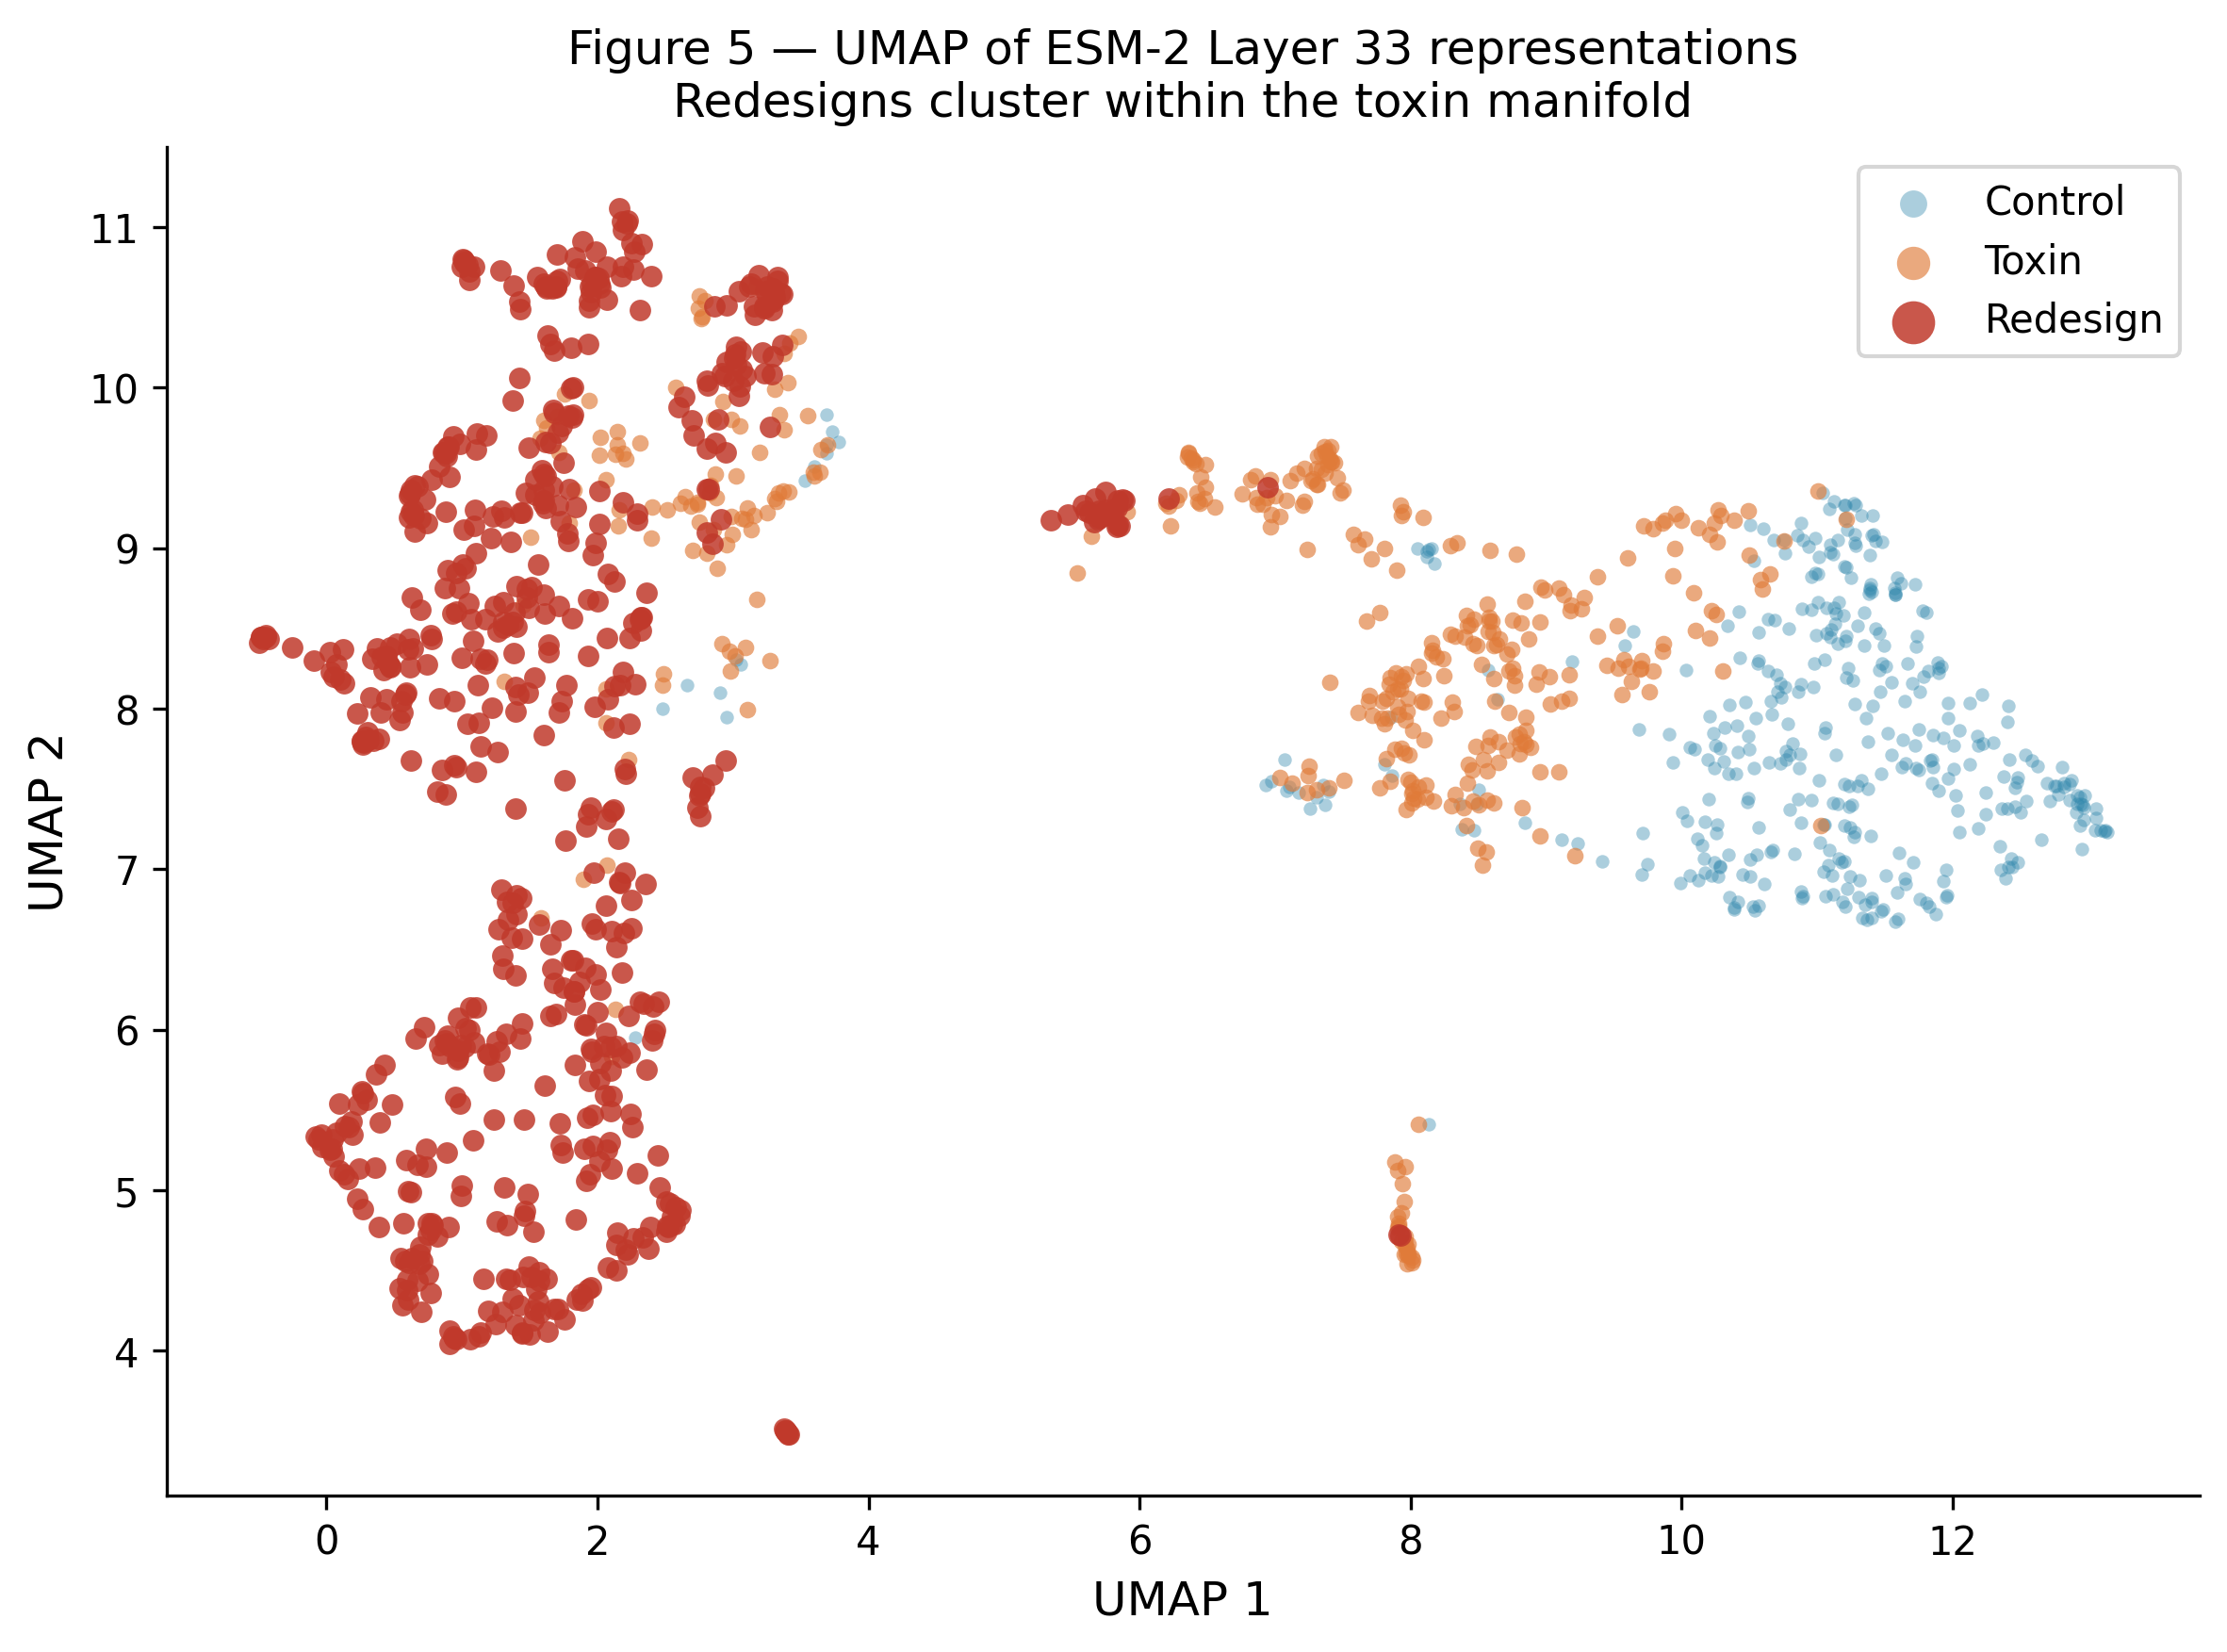
\includegraphics[width=0.8\textwidth]{figures/fig5_umap.png}
    \caption{UMAP projection of embeddings, visualizing the separation between Toxins and Controls, while Redesigns cluster closely with Natural Toxins due to structural preservation.}
\end{figure}

Evadable features encode high-Cys peripheral patterns (C: 3.3--4.7$\times$ enrichment) that ProteinMPNN freely randomises. Robust features split into core disulfide features (C: 1.3--2.6$\times$, transfer 1.67--3.75) and scaffold rigidity features (Pro/Glu, transfer 2.19--3.36). ProteinMPNN preserves both because they are structurally necessary for the toxin fold.

\section{Discussion}

\subsection{Why ProteinMPNN Fails to Evade ESM-2}

ProteinMPNN optimises sequence identity reduction while preserving protein structure. Structure is precisely what ESM-2's toxin circuit encodes. The 8 structure-robust SAE features (transfer ratio 1.4--3.75) fire more strongly on redesigns than natural toxins --- ProteinMPNN's structural preservation \textit{activates} the circuit more reliably than the original sequence diversity.

The 4 sequence-evadable features (transfer < 0.13) show that ProteinMPNN does successfully evade some detection cues. But the probe uses 50 features, and the 8 robust ones suffice to maintain 86--88\% sensitivity.

\subsection{SAE--Probe Geometric Analysis}

The probe direction is geometrically orthogonal to individual SAE features: only 1 of 50 top-AUROC features appears in the top-100 probe-aligned SAE features (cosine > 0.33).

The most probe-aligned SAE feature (F8284, cosine = +0.501) is also the most evadable (transfer = 0.015) --- ProteinMPNN successfully eliminates the sequence pattern this feature detects. This explains the 8.2\% random evasion gap.

Structurally-robust features (F6122, F4097, F1055) have low individual probe alignment (+0.01 to +0.19) but activate at 55--99\% rate in redesigns. The probe's 88\% detection is therefore a \textit{collective} property: no single feature is responsible, and no single redesign operation can eliminate all structural signals simultaneously.

This is consistent with the superposition hypothesis: the probe extracts a direction encoding toxin function that is spread across many weakly-aligned SAE features rather than concentrated in any single one.

\subsection{The Circuit Architecture}

ESM-2 computes toxin function through a distributed progressive representation:
\begin{enumerate}
    \item \textbf{Early layers (1--9)}: Sequence-level features begin accumulating (layer sweep AUROC 0.97 by L9)
    \item \textbf{Mid layers (17--20)}: Primary toxin discrimination builds (DPA +40--45 per layer)
    \item \textbf{Suppressor layers (27--28)}: Internal regulation reduces false positives
    \item \textbf{Final layers (29--32)}: Strong final-phase discrimination (DPA +23--130)
    \item \textbf{Calibration layer (33)}: Large opposing correction normalises the signal
\end{enumerate}

\begin{figure}[H]
    \centering
    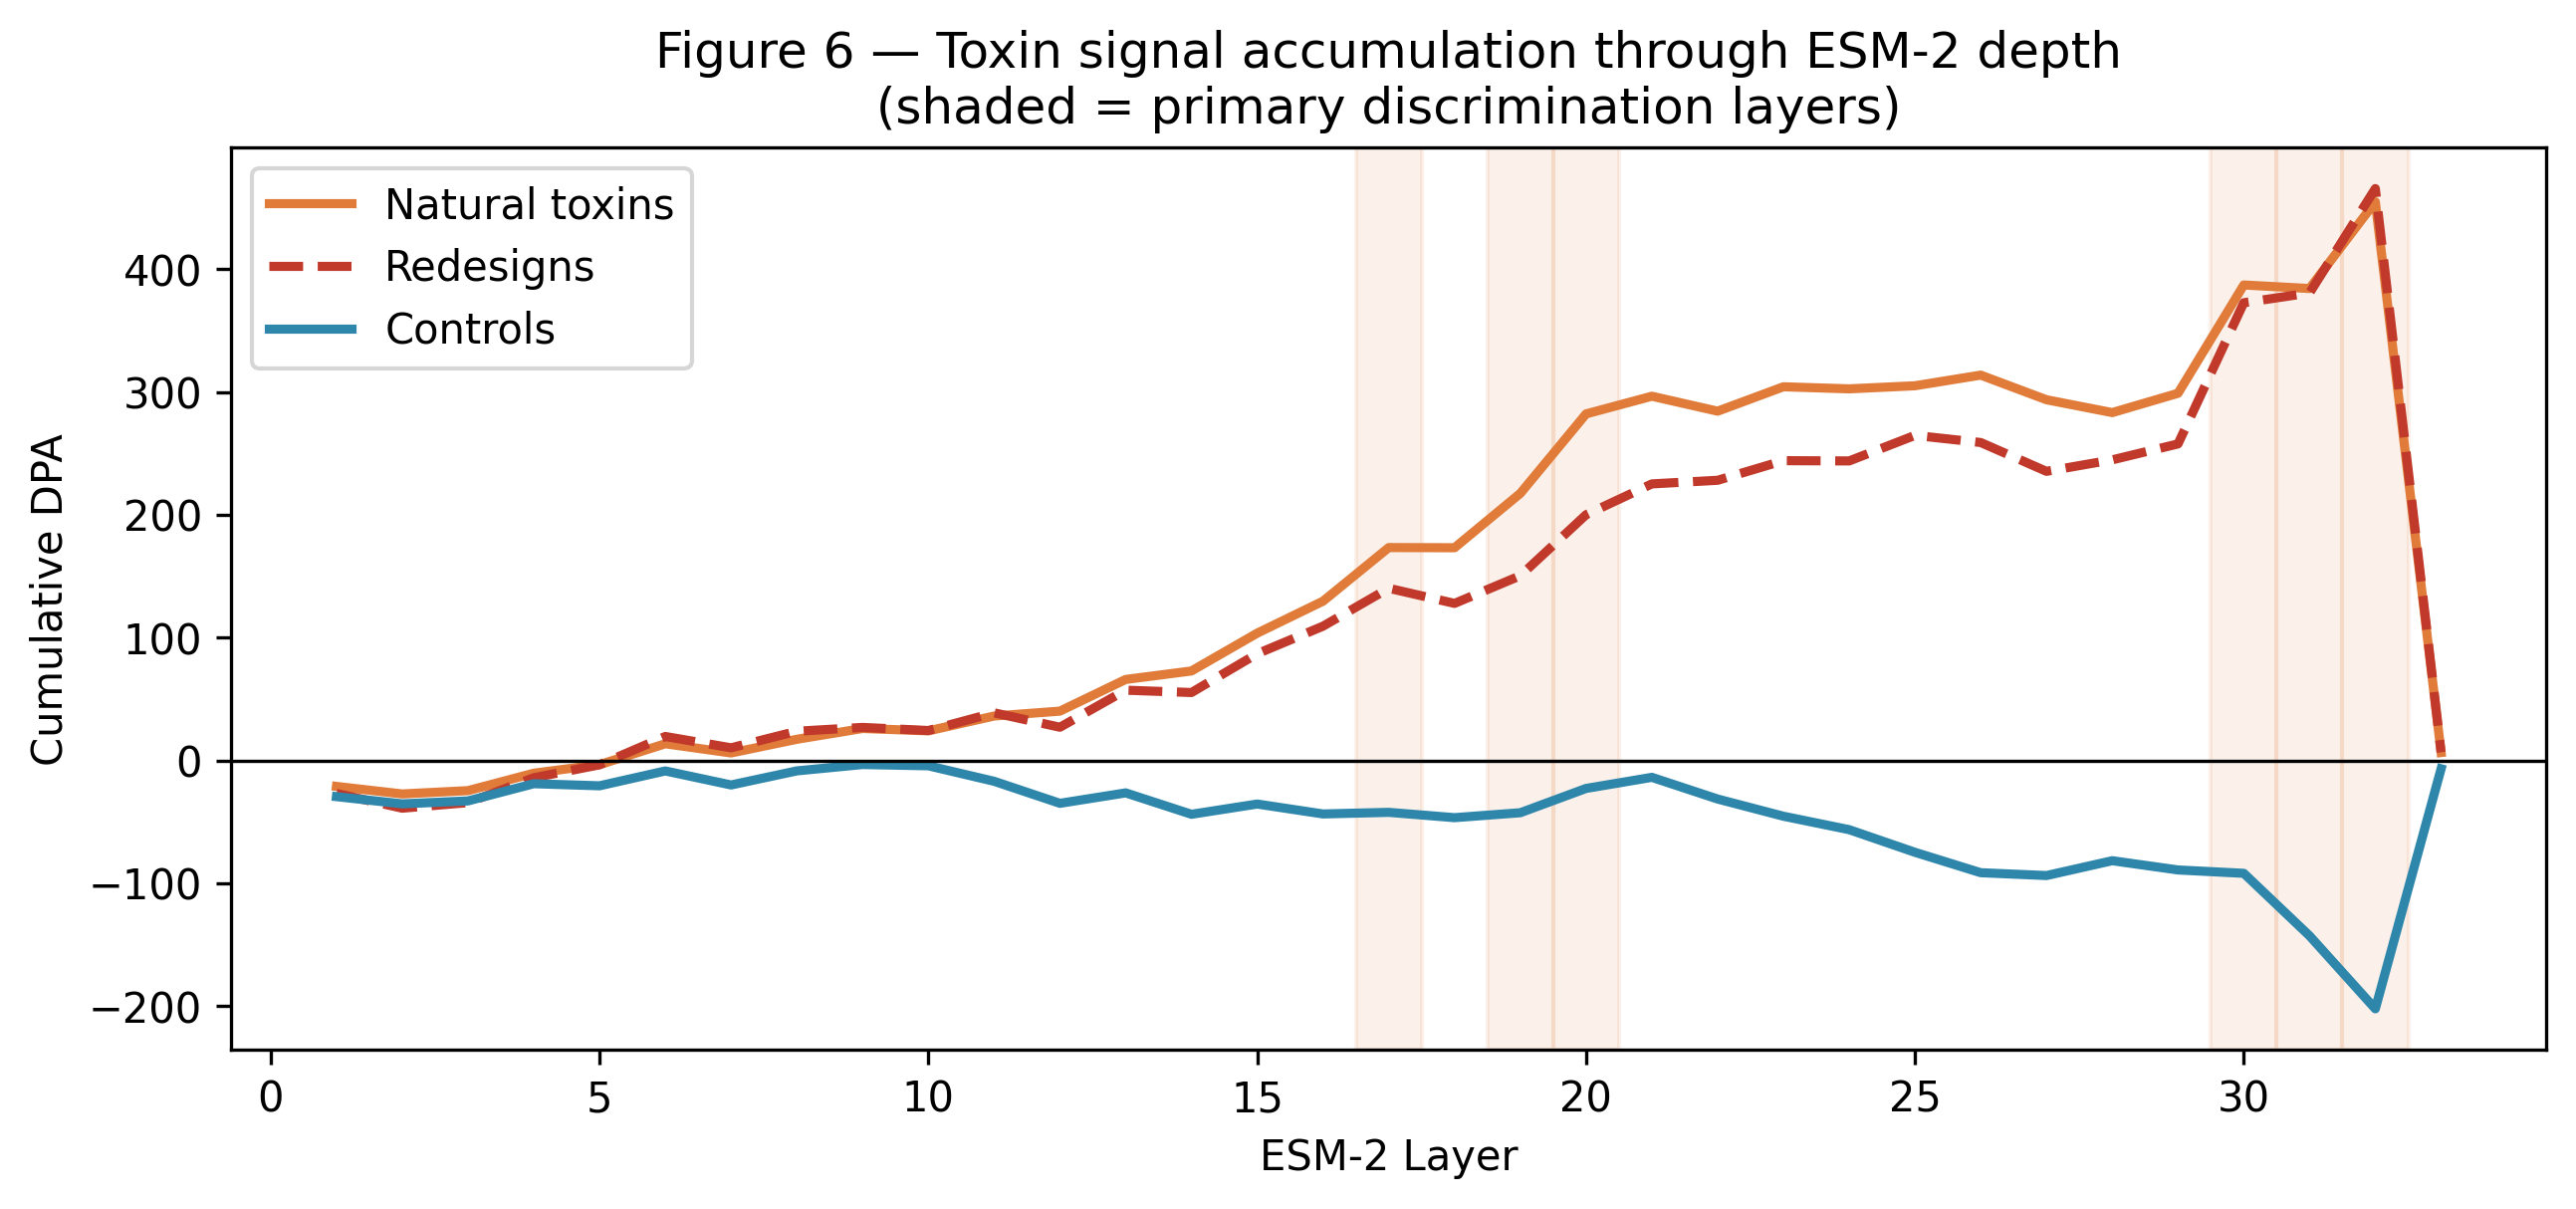
\includegraphics[width=0.8\textwidth]{figures/fig6_dpa_trajectory.png}
    \caption{Cumulative DPA trajectory showing toxin signal accumulation through ESM-2 depth. Natural toxins and ProteinMPNN redesigns follow a nearly identical attribution path, confirming they activate the same distributed circuit.}
\end{figure}

This architecture explains why single-layer activation patching recovers at most 16\% --- the toxin signal requires the full computation graph.

\subsection{Biosecurity Implications}

\begin{enumerate}
    \item \textbf{Sequence-based screening is insufficient}: All 723 ProteinMPNN redesigns evade BLAST at every threshold.
    \item \textbf{ESM-2 probes are robust by architecture}: The toxin circuit uses distributed structural features that sequence redesign preserves.
    \item \textbf{The probe does not require knowledge of redesigns}: 88\% detection with no retraining on any redesigned sequence.
    \item \textbf{Sequence-evadable features exist} (4/20 top features, transfer < 0.13): A more targeted attack could attempt to suppress these. But the remaining 8 robust features maintain detection.
\end{enumerate}

\subsection{Limitations}
\begin{itemize}
    \item \textbf{Embedding-space only}: Our analysis operates on ESM-2 embeddings, not raw sequences. Sequence-space adversarial attacks require ESM-2 inversion.
    \item \textbf{No wet-lab validation}: We cannot confirm redesigned sequences retain toxin function.
    \item \textbf{Single redesign tool}: Analysis covers ProteinMPNN only; RFdiffusion and EvoDiff may produce different identity/transfer profiles.
    \item \textbf{Small $n$ for patching}: DLA computed on 15 pairs; replication on larger sets recommended.
\end{itemize}

\section{Conclusions}

We built the first mechanistic interpretability pipeline for biosecurity, analysing ESM-2's toxin detection against ProteinMPNN adversarial redesigns. Our findings:

\begin{itemize}
    \item \textbf{BLAST: 0\%. ESM-2: 88\%.} ProteinMPNN fails to evade structure-aware probes.
    \item \textbf{205$\times$ compression}: 50 SAE features replicate full-embedding AUROC (0.944 vs 0.959).
    \item \textbf{Transfer ratio 1.28}: Redesigns amplify toxin features on average; 8 of top-20 features activate at > 55\% rate in redesigns.
    \item \textbf{r = 0.992}: Redesigns use the same DLA circuit as natural toxins (layers 17--20, 29--32).
    \item \textbf{Distributed circuit}: No single bottleneck layer; full depth required for 88\% detection.
\end{itemize}

The key insight: ProteinMPNN cannot redesign away what is structurally necessary for toxin function. ESM-2's toxin circuit encodes precisely those structural features.

\subsection{Software Artifacts Delivered}

To translate these mechanistic findings into actionable biosecurity infrastructure, we have developed and open-sourced two software artifacts:
\begin{enumerate}
    \item \textbf{\texttt{screen.py}}: A deployable, zero-shot CLI tool that screens FASTA sequences for toxic function using our structural probe. It provides probability scores, risk levels, and (via an \texttt{--explain} flag) the layer-wise DPA attribution for transparent decision-making.
    \item \textbf{\texttt{demo.ipynb}}: An interactive Jupyter notebook that allows users to test the screening pipeline and visualize the exact layers driving the model's classification.
\end{enumerate}

\section*{Key Numbers Reference}

\begin{table}[H]
\centering
\begin{tabular}{lc}
\toprule
\textbf{Metric} & \textbf{Value} \\
\midrule
Training toxins & 1,712 \\
Training controls & 2,072 \\
ProteinMPNN redesigns & 723 \\
Best probe layer & 33 \\
Probe AUROC (natural test) & 0.9970 \\
BLAST detection on redesigns & \textbf{0.0\%} \\
ESM-2 detection on redesigns & \textbf{88.3\%} \\
SAE features total & 10,240 \\
Dead SAE features & 8,345 (81.5\%) \\
Top-K features used & 50 \\
Compression ratio & 205$\times$ \\
SAE AUROC (top-50) & 0.9447 \\
Mean transfer ratio & \textbf{1.28} \\
Steering (ctrl baseline) & 0.046 \\
Steering (at $+3\sigma$) & \textbf{1.000} \\
Redesign probe score (baseline) & 0.857 \\
DPA tox/redesign correlation & \textbf{$r = 0.992$} \\
Primary discrimination layers & 17--20, 29--32 \\
Max patching recovery & 0.16 \\
\bottomrule
\end{tabular}
\end{table}

\end{document}
